\section{Procesy i zarządzanie procesami}

\subsection{Wstęp}

Przykłady procesów w życiu codziennym: proces fizyczny, chemiczny,
technologiczny, proces sądowy, administracyjny. Proces to przebieg powiązanych
ze sobą zmian. Większość procesów zachodzi w~określonym środowisku (np.
w~urzędzie), podlega pewnym ograniczeniom (np.  procedurom prawnym) i~wymaga
pewnych zasobów (np.  pieniędzy podatników). Pewne zdarzenia w~procesie
mogą występować sekwencyjnie, inne mogą nakładać się na siebie w~czasie. Jeśli
jesteśmy w~stanie wyodrębnić unikalny ciąg występujących po sobie zdarzeń
powiązanych tak, że ich przestawienie czy uniezależnienie od siebie jest
niemożliwe, bądź przeczyłoby logice, to taką sekwencję często określa się
mianem wątku. Proces, podobnie jak fabuła powieści, może obejmować wiele wątków
biegnących równocześnie.

Niektóre z~wymienionych faktów mają przeniesienie na procesy w~systemach
operacyjnych. Proces działa w~środowisku systemu operacyjnego, podlega
restrykcjom narzucanym przez system operacyjny (np. ograniczenia dostępu do
cudzych plików). Procesowi przydzielane są zasoby takie jak czas procesora,
obszar pamięci operacyjnej, pliki, urządzenia peryferyjne. W~pamięci komputera
zwykle znajduje się wiele procesów, które są na różnych etapach wykonania
i~współzawodniczą o~zasoby. W~obrębie jednego procesu występuje jeden lub
więcej wątków (w uproszczeniu wątek obrazuje ciąg wykonywanych po sobie
instrukcji), wątki mogą być wykonywane równolegle

Proces, jak większość obiektów w~informatyce, posiada pewne atrybuty, można na
nim dokonywać pewnych operacji (funkcje) oraz podlega regułom określającym jego
czas życia. W~niniejszym laboratorium omówimy następujące zagadnienia:
\begin{myitemize}
  \item wyświetlanie i~modyfikowanie atrybutów procesów (atrybuty),
  \item funkcje umożliwiające tworzenie i usuwanie procesów (czas życia).
\end{myitemize}

Często proces jest utożsamiany z~programem uruchomionym w~systemie operacyjnym.
Rzeczywiste aplikacje mogą się jednak składać z~wielu procesów. W~niniejszym
laboratorium zostaną pokazane przykłady prostych aplikacji wielo-procesowych
zapisanych w~języku C.

\subsection{Wyświetlanie i modyfikowanie atrybutów procesów}

Atrybuty to pewne właściwości przypisane procesowi. Każdy proces w systemie QNX
ma np. przypisany unikalny identyfikator PID (process ID), który jest liczbą
całkowitą. Każdy proces (oprócz procesu ,,głównego'' \texttt{procnto}) ma
również swój proces macierzysty. Identyfikator PPID (parent process ID) jest
identyfikatorem PID procesu macierzystego. Proces \texttt{procnto} ma
identyfikator PID=1. Wybrane atrybuty i~funkcje systemowe umożliwiające dostęp
do nich przedstawiono w~tabeli \ref{tab:HE6LE}.

%%%%%%%%%%%%%%%%%%%%%%%%%%%%%%%%%%%%%%%%%%%%%%%%%%%%%%%%%%%%%%%%%%%%%%%%%%%%%
\begin{table}[h!]
  \centering
  \caption{Niektóre atrybuty procesów oraz funkcje biblioteki systemowej
           umożliwiające dostęp do nich}
  \label{tab:HE6LE}
  \begin{tabular}{|c|c|c|}
    \hline
    \textbf{Atrybuty procesu} & \textbf{Wyświetlanie} & \textbf{Modyfikacja} \\ \hline
    Identyfikator PID                   & \texttt{getpid()}           & -- \\ \hline
    Identyfikator PPID                  & \texttt{getppid()}          & -- \\ \hline
    Priorytet i~strategia szeregowania  & \texttt{sched\_getparam()}  & \texttt{sched\_setparam()} \\ \hline
  \end{tabular}
\end{table}
%%%%%%%%%%%%%%%%%%%%%%%%%%%%%%%%%%%%%%%%%%%%%%%%%%%%%%%%%%%%%%%%%%%%%%%%%%%%%

Na ogół mamy do czynienia z sytuacją, kiedy procesów gotowych do wykonania jest
więcej niż umożliwiają to dostępne w~danej chwili zasoby. Procedura szeregująca
(scheduler) rozstrzyga, któremu z procesów (wątków) zostanie w~danej chwili
przydzielony czas procesora. Jednym z~istotnych parametrów rzutujących na
kolejność przydzielania czasu procesora jest priorytet -- każdy z procesów (i
wątków -- patrz następne laboratoria) ma przyporządkowany priorytet (process
priority).  Jest on miarą pilności wykonania danego procesu względem innych.
W systemie QNX Neutrino 6 priorytet jest liczbą z zakresu od 0 (najniższy) do
255 (najwyższy). System nakłada ograniczenia na dopuszczalne zakresy
priorytetów dla programów uruchamianych przez poszczególnych użytkowników
(tabela \ref{tab:2N6W7}):

%%%%%%%%%%%%%%%%%%%%%%%%%%%%%%%%%%%%%%%%%%%%%%%%%%%%%%%%%%%%%%%%%%%%%%%%%%%%%
\begin{table}[h!]
  \centering
  \caption{Priorytety w~QNX Neutrino 6}
  \label{tab:2N6W7}
  \begin{tabular}{|c|c|c|}
    \hline
    \textbf{Priorytet} & \textbf{Użytkownik} \\ \hline
    0 & Proces jałowy \\ \hline
    1 -- 63 & Wątki zwykłego użytkownika \\ \hline
    1 -- 255 & Wątki użytkownika \texttt{root} \\ \hline
  \end{tabular}
\end{table}
%%%%%%%%%%%%%%%%%%%%%%%%%%%%%%%%%%%%%%%%%%%%%%%%%%%%%%%%%%%%%%%%%%%%%%%%%%%%%

W systemie QNX są dostępne trzy strategie szeregowania:
\begin{myitemize}
  \item szeregowanie FIFO (FIFO scheduling),
  \item szeregowanie karuzelowe (round robin scheduling),
  \item szeregowanie sporadyczne (sporadic scheduling).
\end{myitemize}
Są one omówione szczegółowo w dokumentacji QNX~\cite{qnx}. W tabeli
\ref{tab:A9C2X} przedstawiono ich symbole, wykorzystywane w~wywołaniach
systemowych (symbole te zdefiniowane są w~pliku nagłówkowym \texttt{sched.h}).

%%%%%%%%%%%%%%%%%%%%%%%%%%%%%%%%%%%%%%%%%%%%%%%%%%%%%%%%%%%%%%%%%%%%%%%%%%%%%
\begin{table}[h!]
  \centering
  \caption{Strategie szeregowania w~QNX Neutrino 6}
  \label{tab:A9C2X}
  \begin{tabular}{|c|c|c|}
    \hline
    \textbf{Symbol}           & \textbf{Opis} \\ \hline
    \texttt{SCHED\_FIFO}      & Szeregowanie FIFO \\ \hline
    \texttt{SCHED\_RR}        & Szeregowanie karuzelowe \\ \hline
    \texttt{SCHED\_SPORADIC}  & Szeregowanie sporadyczne \\ \hline
  \end{tabular}
\end{table}
%%%%%%%%%%%%%%%%%%%%%%%%%%%%%%%%%%%%%%%%%%%%%%%%%%%%%%%%%%%%%%%%%%%%%%%%%%%%%

%%%%%%%%%%%%%%%%%%%%%%%%%%%%%%%%%%%%%%%%%%%%%%%%%%%%%%%%%%%%%%%%%%%%%%%%%%%%%
\begin{example}{[Lista procesów]}
  \label{ex:TYRDA}
  W terminalu wykonać polecenie \texttt{ps -l}. Sprawdzić w {\color{red}dokumentacji},
  co oznaczają poszczególne kolumny wyświetlonego raportu.
\end{example}
%%%%%%%%%%%%%%%%%%%%%%%%%%%%%%%%%%%%%%%%%%%%%%%%%%%%%%%%%%%%%%%%%%%%%%%%%%%%%

%%%%%%%%%%%%%%%%%%%%%%%%%%%%%%%%%%%%%%%%%%%%%%%%%%%%%%%%%%%%%%%%%%%%%%%%%%%%%
\begin{example}{[Wyświetlanie i modyfikacja wybranych atrybutów procesu]}
  \label{ex:TEPBG}
  \lstinputlisting[style=MyCStyle,label=src:4JKQ7]{src/lab4/attributes1.c}
\end{example}
%%%%%%%%%%%%%%%%%%%%%%%%%%%%%%%%%%%%%%%%%%%%%%%%%%%%%%%%%%%%%%%%%%%%%%%%%%%%%


\subsection{Tworzenie procesów}

W systemie QNX Neutrino, modułem odpowiedzialnym za dynamiczne tworzenie,
usuwanie oraz zarządzanie procesami jest zawarty w mikrojądrze (procnto)
manager procesów. W systemie QNX istnieją różne metody tworzenia procesów.
Część z nich pochodzi wprost od systemów UNIX-owych, opartych o standard POSIX,
inne funkcje do tworzenia procesów są charakterystyczne tylko dla systemu QNX.
Podstawowe funkcje do tworzenia procesów przedstawiono w tabeli
\ref{tab:IMJR3}. W ramach laboratorium omówimy cztery funkcje służące
tworzeniu procesów, tj. \texttt{system()}, \texttt{fork()}, \texttt{exec()},
\texttt{spawn()}.

%%%%%%%%%%%%%%%%%%%%%%%%%%%%%%%%%%%%%%%%%%%%%%%%%%%%%%%%%%%%%%%%%%%%%%%%%%%%%
\begin{table}[h!]
  \centering
  \caption{Metody tworzenia procesów w systemie QNX}
  \label{tab:IMJR3}
  \begin{tabular}{|l|p{0.75\textwidth}|}
    \hline
    \textbf{Funkcja}    & \textbf{Opis}  \\ \hline
    \texttt{system()}   & Wywołanie programów, poleceń systemowych, bądź skryptów \\ \hline
    \texttt{fork()}     & Utworzenie kopii procesu bieżącego \\ \hline
    \texttt{exec()}     & Zastąpienie bieżącego procesu nowym procesem -- rodzina funkcji \\ \hline
    \texttt{spawn()}    & Utworzenie procesu potomnego -- rodzina funkcji \\ \hline
    \texttt{vfork()}    & Utworzenie procesu potomnego i zablokowanie procesu macierzystego \\ \hline
    \texttt{forkpty()}  & Utworzenie procesu potomnego w oknie pseudoterminala \\ \hline
    \texttt{popen()}    & Uruchomienie programu jako procesu potomnego z
                          jednoczesnym utworzeniem łącza pomiędzy procesem
                          bieżącym, a potomnym \\ \hline
  \end{tabular}
\end{table}
%%%%%%%%%%%%%%%%%%%%%%%%%%%%%%%%%%%%%%%%%%%%%%%%%%%%%%%%%%%%%%%%%%%%%%%%%%%%%

Jeden ze sposobów na utworzenie nowego procesu polega na uruchomieniu programu
zapisanego w~pliku wykonywalnym. Z~poziomu języka C można tego dokonać używając
funkcji \texttt{system()} (przykład \ref{ex:V86MA}). Poleceniem tym można
uruchomić program w~sposób podobny, jak to się czyni wprost z~powłoki. Funkcja
zwraca status zakończenia uruchomionego programu.

%%%%%%%%%%%%%%%%%%%%%%%%%%%%%%%%%%%%%%%%%%%%%%%%%%%%%%%%%%%%%%%%%%%%%%%%%%%%%
\begin{example}{[Wywołanie programu za pomocą polecenia system()]}
  \label{ex:V86MA}
  \lstinputlisting[style=MyCStyle,label=src:P1A10]{src/lab4/system1.c}
\end{example}
%%%%%%%%%%%%%%%%%%%%%%%%%%%%%%%%%%%%%%%%%%%%%%%%%%%%%%%%%%%%%%%%%%%%%%%%%%%%%

Funkcja \texttt{fork()} tworzy kopię bieżącego procesu i~uruchamia ją jako
proces potomny. Utworzony proces potomny wykonuje się współbieżnie z procesem
tworzącym, posiada własny nr PID, a jego PPID wskazuje na proces tworzący.
Funkcja \texttt{fork()} tworzy deskryptor nowego procesu oraz kopię segmentu
kodu, danych i stosu. Modyfikacje zmiennych w procesie macierzystym nie są
widoczne w procesie potomnym i odwrotnie. Jeżeli operacja utworzenia procesu
potomnego zakończy się powodzeniem, to funkcja w procesie macierzystym zwraca
identyfikator (PID) procesu potomnego (wartość większa od 1), a w procesie
potomnym wartość 0. W~przypadku niepowodzenia, funkcja \texttt{fork()} zwraca
wartość \texttt{-1}. Działanie funkcji przedstawiono na rysunku
\ref{fig:S278F}, a użycie w przykładzie~\ref{ex:HP9M8}.

%%%%%%%%%%%%%%%%%%%%%%%%%%%%%%%%%%%%%%%%%%%%%%%%%%%%%%%%%%%%%%%%%%%%%%%%%%%%%
\begin{figure}
  \centering
  \begin{tikzpicture}
    \node[TBox6emCentered] (parent)   at (0.00,3.50)  {Proces macierzysty};
    \node                  (fork)     at (0.00,1.75)  {\texttt{fork()}};
    \node                  (x)        at (4.50,1.75)  {};
    \node[TBox6emCentered] (parent2)  at (0.00,0.00)  {Proces macierzysty};
    \node[TBox6emCentered] (child)    at (4.50,0.00)  {Proces potomny};

    \draw[->] (parent.south)  to                                                (fork.north);
    \draw[->] (fork.south)    to node[anchor=center,left]{Zwraca PID potomka}   (parent2.north);
    \draw[->] (fork.east)     to                                                (x.center)
                              to node[anchor=center, right]{Zwraca zero}        (child.north);
  \end{tikzpicture}
  \caption{Idea działania funkcji \texttt{fork()}}
  \label{fig:S278F}
\end{figure}
%%%%%%%%%%%%%%%%%%%%%%%%%%%%%%%%%%%%%%%%%%%%%%%%%%%%%%%%%%%%%%%%%%%%%%%%%%%%%

%%%%%%%%%%%%%%%%%%%%%%%%%%%%%%%%%%%%%%%%%%%%%%%%%%%%%%%%%%%%%%%%%%%%%%%%%%%%%
\begin{example}{[Wywołanie funkcji fork()]}
  \label{ex:HP9M8}
  \lstinputlisting[style=MyCStyle,label=src:Z5EXB]{src/lab4/fork1.c}

  Sprawdzić działanie programu, gdy zmienna CHILD = 8, a zmienna PARENT = 4.
\end{example}
%%%%%%%%%%%%%%%%%%%%%%%%%%%%%%%%%%%%%%%%%%%%%%%%%%%%%%%%%%%%%%%%%%%%%%%%%%%%%

\subsection{Obsługa zakończenia procesów}

Procesy na ogół współdziałają ze sobą (np. komunikują się), mogą też być
w~relacji pokrewieństwa (dany proces może być np. procesem macierzystym innych
procesów). Proces może, dla przykładu, oczekiwać na określone zdarzenia,
generowane przez inne procesy. Przedwczesne lub nieprawidłowe zakończenie
procesu, będącego częścią aplikacji wielo-procesowej, może doprowadzić do
błędów w~działaniu aplikacji lub niepotrzebnego zużycia zasobów systemowych.
Przed zakończeniem procesu należy zwolnić zajęte przezeń zasoby, zakończyć z
innymi procesami scenariusze komunikacyjne i~synchronizacyjne, a w~przypadku
procesów macierzystych, zaczekać na zakończenie procesów potomnych.

Zakończenie procesu jest inicjowane w~następujących sytuacjach:
\begin{myitemize}
  \item wywołaniem funkcji \texttt{exit()} z~poziomu procesu,
  \item poprzez powrót z~funkcji \texttt{main()}, np. instrukcją \texttt{return},
  \item proces zakończony/unicestwiony przez system operacyjny lub inny proces.
\end{myitemize}

W~dowolnym miejscu programu można zainicjować zakończenie procesu funkcją \texttt{exit()}
%%%%%%%%%%%%%%%%%%%%%%%%%%%%%%%%%%%%%%%%%%%%%%%%%%%%%%%%%%%%%%%%%%%%%%%%%%%%%
\begin{lstlisting}[style=MyCStyle]
 #include <stdlib.h>
 void exit( int status );
\end{lstlisting}
%%%%%%%%%%%%%%%%%%%%%%%%%%%%%%%%%%%%%%%%%%%%%%%%%%%%%%%%%%%%%%%%%%%%%%%%%%%%%
Funkcja ta powoduje zakończenie procesu bieżącego oraz przekazanie do procesu
macierzystego wartości \texttt{status}. Przyjęło się przekazywać wartość
\texttt{EXIT\_SUCCESS}, gdy proces zakończył się poprawnie, bądź
\texttt{EXIT\_FAILURE}, gdy wystąpił błąd (to samo dotyczy instrukcji
\texttt{return} w~funkcji \texttt{main}).

Jeśli dany proces posiada potomków, należy zapobiegać tzw. ,,osieracaniu
procesów''. Ma to miejsce gdy proces macierzysty kończy się wcześniej niż jego
procesy potomne. Proces macierzysty powinien zaczekać na zakończenie wszystkich
swoich procesów potomnych. Można do tego użyć funkcji \texttt{wait()}:
%%%%%%%%%%%%%%%%%%%%%%%%%%%%%%%%%%%%%%%%%%%%%%%%%%%%%%%%%%%%%%%%%%%%%%%%%%%%%
\begin{lstlisting}[style=MyCStyle]
  #include <sys/types.h>
  #include <sys/wait.h>
  pid_t wait( int * status );
\end{lstlisting}
%%%%%%%%%%%%%%%%%%%%%%%%%%%%%%%%%%%%%%%%%%%%%%%%%%%%%%%%%%%%%%%%%%%%%%%%%%%%%
Funkcja \texttt{wait()} wstrzymuje bieżący proces do momentu zakończenia
któregokolwiek z~jego procesów potomnych. Funkcja zwraca PID zakończonego
procesu (bądź \texttt{-1}, gdy brak procesów potomnych). Pod adres wskazany
przez argument \texttt{status} wpisywany jest status zakończenia procesu. Ten
\texttt{status} zawiera liczbę \texttt{status} podaną w~procesie potomnym do
funkcji \texttt{exit()} bądź instrukcji \texttt{return}, ale wartość ta może
być w~pewien sposób ,,zakodowana''. Do jej ,,odkodowania'' używa się makra
\texttt{WEXITSTATUS()}.

%%%%%%%%%%%%%%%%%%%%%%%%%%%%%%%%%%%%%%%%%%%%%%%%%%%%%%%%%%%%%%%%%%%%%%%%%%%%%
\begin{figure}
  \centering
  \begin{tikzpicture}
    \node[TBox6emCentered]  (parent)  at (0.00, 3.50) {Proces macierzysty};
    \node                   (fork)    at (0.00, 2.00) {\texttt{fork()}};
    \node                   (wait)    at (0.00, 0.75) {\texttt{wait()}};
    \node[TBox6emCentered]  (child)   at (4.50, 2.00) {Proces potomny};
    \node[circle,draw=black](o)       at (0.00,-0.25) {};
    \node                   (exit)    at (4.50,-0.25) {\texttt{exit()}};
    \node                   (end1)    at (0.00,-1.00) {};
    \node[circle,fill=black](end2)    at (4.50,-1.00) {};
    \node[right of = end2]  (end2t)   {Koniec};

    \draw[->] (parent.south)  to (fork.north);
    \draw[->] (fork.east)     to (child.west);
    \draw[->] (fork.south)    to (wait.north);
    \draw[->] (wait.south)    to node[anchor=center,left]{Oczekiwanie} (o.north);
    \draw[->] (child.south)   to (exit.north);
    \draw[->,dotted] (exit.west)     to (o.east);
    \draw[->] (o.south)       to node[anchor=center,left]{Dalszy bieg} (end1.south);
    \draw[->] (exit.south)    to (end2);
  \end{tikzpicture}
  \caption{Schemat poprawnego zakończenia procesu}
  \label{fig:Z6B8G}
\end{figure}
%%%%%%%%%%%%%%%%%%%%%%%%%%%%%%%%%%%%%%%%%%%%%%%%%%%%%%%%%%%%%%%%%%%%%%%%%%%%%

Ilustrację omawianych zagadnień stanowi przykład \ref{ex:11SSB}. Zastosowanie
funkcji \texttt{wait()} w~przykładzie \ref{ex:11SSB} powoduje, że proces
macierzysty nie zakończy się przed procesem potomnym.
%%%%%%%%%%%%%%%%%%%%%%%%%%%%%%%%%%%%%%%%%%%%%%%%%%%%%%%%%%%%%%%%%%%%%%%%%%%%%
\begin{example}{[Wywołanie funkcji fork() wraz z obsługą zakończenia procesów]}
  \label{ex:11SSB}
  \lstinputlisting[style=MyCStyle,label=src:92W6D]{src/lab4/process1.c}
\end{example}
%%%%%%%%%%%%%%%%%%%%%%%%%%%%%%%%%%%%%%%%%%%%%%%%%%%%%%%%%%%%%%%%%%%%%%%%%%%%%

Możliwy jest scenariusz, w~którym proces potomny zainicjuje swoje zakończenie
zanim proces macierzysty ,,dobiegnie'' do funkcji \texttt{wait()}. Zwalniane są
wtedy wtedy wszystkie zasoby procesu potomnego, z wyjątkiem deskryptora
procesu, czyli miejsca w pamięci operacyjnej, gdzie przechowywane są informacje
potrzebne do zarządzania procesem. Tam zapamiętywany jest m.in. status
zakończenia procesu potomnego, który ma być przekazany do procesu
macierzystego. Proces oczekuje w~rekordach systemowych na zwolnienie
deskryptora, które może być dokonane dopiero po wywołaniu \texttt{wait()} przez
proces macierzysty. Taki stan procesu potomnego nazywa się stanem ,,zombie''.

Do oczekiwania na zakończenie \textit{konkretnego} procesu można użyć funkcji
\texttt{waitpid()}.
%%%%%%%%%%%%%%%%%%%%%%%%%%%%%%%%%%%%%%%%%%%%%%%%%%%%%%%%%%%%%%%%%%%%%%%%%%%%%
\begin{lstlisting}[style=MyCStyle]
#include <sys/types.h>
#include <sys/wait.h>

pid_t waitpid( pid_t pid, int *status, int options );
\end{lstlisting}
%%%%%%%%%%%%%%%%%%%%%%%%%%%%%%%%%%%%%%%%%%%%%%%%%%%%%%%%%%%%%%%%%%%%%%%%%%%%%
Funkcja zwraca PID zakończonego procesu, bądź \texttt{-1}, w przypadku, gdy
brak jest procesów potomnych. Funkcja zwraca również status zakończonego
procesu poprzez argument \texttt{status}. Jedną z użytecznych opcji
(\texttt{options}) jest flaga \texttt{WNOHANG}, która powoduje, że proces
macierzysty, w przypadku braku oczekujących procesów potomnych, natychmiast
wraca z funkcji i kontynuuje swoje działanie i w tym przypadku możemy użyć
takiej kombinacji do cyklicznego sprawdzania, czy proces potomny się zakończył.


\subsection{Zastąpienie procesu bieżącego innymi procesami}

Funkcje z rodziny \texttt{exec()} zastępują bieżący proces nowym procesem,
powstałym poprzez uruchomienie wskazanego pliku wykonywalnego. W~systemie QNX
zdefiniowano następującą rodzinę funkcji: \texttt{execl()}, \texttt{execle()},
\texttt{execlp()}, \texttt{execlpe()}, \texttt{execv()}, \texttt{execve()},
\texttt{execvp()}, \texttt{execvpe()}. Działanie tych funkcji jest podobne,
natomiast różnią się listą parametrów formalnych. W trakcie laboratorium
będziemy używać najprostszych funkcji \texttt{execl()} oraz \texttt{execv()},
o~następujących sygnaturach:
%%%%%%%%%%%%%%%%%%%%%%%%%%%%%%%%%%%%%%%%%%%%%%%%%%%%%%%%%%%%%%%%%%%%%%%%%%%%%
\begin{lstlisting}[style=MyCStyle]
#include <process.h>

int execl(  const char * path,
            const char * arg0,
            const char * arg1,
            ...
            const char * argn,
            NULL );
int execv( const char * path,
           char * const argv[] );
\end{lstlisting}
%%%%%%%%%%%%%%%%%%%%%%%%%%%%%%%%%%%%%%%%%%%%%%%%%%%%%%%%%%%%%%%%%%%%%%%%%%%%%
gdzie \texttt{path} jest ścieżką do pliku wykonywalnego, a argumenty
\texttt{arg0} \dots \texttt{argn} (\texttt{argv[0]} \dots \texttt{argv[n]}) --
argumentami przekazanymi do programu. Na ostatnim miejscu podaje się wartość
\texttt{NULL}, na oznaczenie zakończenia listy parametrów wywoływanego
programu. Funkcja \texttt{execl()} nadaje się w~sytuacji, kiedy długość listy
argumentów przekazywanych do uruchamianego programu jest znana już na etapie
programowania aplikacji. Funkcja \texttt{execv()} nadaje się w~sytuacji gdy
długość listy argumentów jest ustalana dopiero w~trakcie działania aplikacji,
np. jest zadana przez użytkownika aplikacji.
%%%%%%%%%%%%%%%%%%%%%%%%%%%%%%%%%%%%%%%%%%%%%%%%%%%%%%%%%%%%%%%%%%%%%%%%%%%%%
\begin{example}{[Wywołanie funkcji execl()]}
  \label{ex:WHF3V}
  \lstinputlisting[style=MyCStyle,label=src:5Y0UB]{src/lab4/execv1.c}
\end{example}
%%%%%%%%%%%%%%%%%%%%%%%%%%%%%%%%%%%%%%%%%%%%%%%%%%%%%%%%%%%%%%%%%%%%%%%%%%%%%

\subsection{Tworzenie procesów funkcją spawn()}

Funkcje z~rodziny \texttt{spawn()}, służą do tworzenia procesów potomnych
poprzez uruchomienie wskazanego pliku wykonywalnego. Do tej grupy zaliczamy
następujące funkcje: \texttt{spawn()}, \texttt{spawnl()}, \texttt{spawnv()},
\texttt{spawnle()}, \texttt{spawnlp()}, \texttt{spawnlpe()},
\texttt{spawnve()}, \texttt{spawnvp()}, \texttt{spawnvpe()}. Omówimy tylko
funkcje \texttt{spawnl()} i~\texttt{spawnv()}, których deklaracje wyglądają
następująco:
%%%%%%%%%%%%%%%%%%%%%%%%%%%%%%%%%%%%%%%%%%%%%%%%%%%%%%%%%%%%%%%%%%%%%%%%%%%%%
\begin{lstlisting}[style=MyCStyle]
#include <process.h>

int spawnl( int mode,
            const char * path,
            const char * arg0,
            const char * arg1,
            ...
            const char * argn,
            NULL );
int spawnv( int mode,
            const char * path,
            char * const argv[] );
\end{lstlisting}
%%%%%%%%%%%%%%%%%%%%%%%%%%%%%%%%%%%%%%%%%%%%%%%%%%%%%%%%%%%%%%%%%%%%%%%%%%%%%
Argument \texttt{mode} jest trybem wykonania procesu, który określa sposób
wywołania procesu potomnego i~zachowanie procesu macierzystego, gdy proces
potomny zostanie zainicjowany (tabela \ref{tab:V0CUU}). Pozostałe argumenty są
interpretowane dokładnie tak samo jak w~przypadku funkcji \texttt{execl()}
i~\texttt{execv()}.

%%%%%%%%%%%%%%%%%%%%%%%%%%%%%%%%%%%%%%%%%%%%%%%%%%%%%%%%%%%%%%%%%%%%%%%%%%%%%
\begin{table}
  \caption{Tryby wywołania funkcji \texttt{spawn()}}
  \label{tab:V0CUU}
  \begin{tabular}{|l|p{0.75\textwidth}|}
    \hline
    \textbf{Tryb}       & \textbf{Opis}
    \\ \hline
    \texttt{P\_WAIT}    & Proces macierzysty czeka na zakończenie procesu
                          potomnego i później jest kontynuowany.
    \\ \hline
    \texttt{P\_NOWAIT}  & Proces macierzysty i potomny są wykonywane
                          współbieżnie. Można używać funkcji \texttt{wait()}.
    \\ \hline
    \texttt{P\_NOWAITO} & Proces macierzysty i potomny są wykonywane
                          współbieżnie. Nie wolno używać funkcji wait() do
                          uzyskania kodu wyjścia. Relacja pokrewieństwa między
                          nimi zostaje przerwana.
    \\ \hline
    \texttt{P\_OVERLAY} & Proces macierzysty jest zastępowany przez proces
                          potomny. Wywołanie w tym trybie jest równoważne
                          wywołaniu funkcji execl().
    \\ \hline
  \end{tabular}
\end{table}
%%%%%%%%%%%%%%%%%%%%%%%%%%%%%%%%%%%%%%%%%%%%%%%%%%%%%%%%%%%%%%%%%%%%%%%%%%%%%

Ilustrację wywołania funkcji \texttt{spawnl()} stanowi przykład \ref{ex:VSCD0}:
%%%%%%%%%%%%%%%%%%%%%%%%%%%%%%%%%%%%%%%%%%%%%%%%%%%%%%%%%%%%%%%%%%%%%%%%%%%%%
\begin{example}{[Wywołanie funkcji spawnl()]}
  \label{ex:VSCD0}
  Utworzyć dwa programy (oddzielne projekty w~środowisku IDE) o~nazwie
  \texttt{macierzysty} i~\texttt{potomny}, następnie wywołać program
  \texttt{macierzysty}.
  \lstinputlisting[style=MyCStyle,label=src:4HNG2]{src/lab4/parent1.c}
  \lstinputlisting[style=MyCStyle,label=src:YZY1R]{src/lab4/child1.c}
\end{example}
%%%%%%%%%%%%%%%%%%%%%%%%%%%%%%%%%%%%%%%%%%%%%%%%%%%%%%%%%%%%%%%%%%%%%%%%%%%%%


\subsection{Ćwiczenia}

\begin{myenumerate}
  \item Napisać program, w~którym proces macierzysty \texttt{P} tworzy dwa
    procesy potomne \texttt{R1}, \texttt{R2}. Każdy z~procesów potomnych
    powinien utworzyć swój własny proces potomny: \texttt{R1} $\to$
    \texttt{S1}, \texttt{R2} $\to$ \texttt{S2}. Każdy z~procesów (z~wyjątkiem
    \texttt{P}) niech wyświetli swój PID oraz PPID.
    \begin{figure}[htbp]
      \centering
      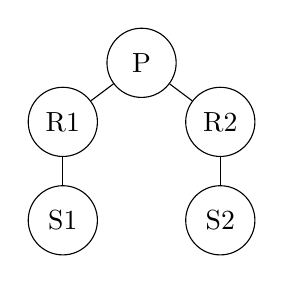
\begin{tikzpicture}
        \node[circle,draw=black,minimum size=2.5em] (P)  at  ( 0.00, 0.00) {P};
        \node[circle,draw=black,minimum size=2.5em] (R1) at  (-1.00,-0.75) {R1};
        \node[circle,draw=black,minimum size=2.5em] (R2) at  ( 1.00,-0.75) {R2};
        \node[circle,draw=black,minimum size=2.5em] (S1) at  (-1.00,-2.00) {S1};
        \node[circle,draw=black,minimum size=2.5em] (S2) at  ( 1.00,-2.00) {S2};

        \draw[-]     (P) to (R1);
        \draw[-]     (P) to (R2);
        \draw[-]     (R1) to (S1);
        \draw[-]     (R2) to (S2);
      \end{tikzpicture}
      \caption{Hierarchia procesów w~ćwiczeniu 1}
      \label{fig:1QZGH}
    \end{figure}
  \item Napisać program, w~którym proces macierzysty \texttt{P} tworzy jeden
    proces potomny \texttt{R} (\texttt{fork()}). Proces \texttt{R} niech
    wyświetli swój PID i uruchomi wskazany plik wykonywalny przy użyciu funkcji
    \texttt{execv()}. Ścieżkę do pliku wykonywalnego oraz argumenty jego
    wywołania przekazać z~wiersza poleceń.
  \item Utworzyć za pomocą funkcji \texttt{fork()} pięć procesów potomnych,
    ponumerowanych (numer kolejny \texttt{i}) od \texttt{0} do \texttt{4}.
    Zaczekać na ich zakończenie. Niech każdy z~procesów potomnych wyświetla
    cyklicznie co jedną sekundę swój \texttt{PID}, numer kolejny \texttt{i},
    oraz numer cyklu. Liczba cykli do wykonania przez poszczególne procesy
    powinny pochodzić z~tablicy zdefiniowanej wewnątrz funkcji \texttt{main()},
    np. \texttt{int t[] = \{20, 5, 3, 8, 9\}}. Na zakończenie procesu potomnego
    o nr \texttt{i} wywołać funkcję \texttt{exit(i)}. Proces macierzysty
    powinien czekać na zakończenie potomnych i wyświetlić \texttt{PID}
    zakończonego procesu oraz wartość podaną przez proces potomny do funkcji
    \texttt{exit()}.
    %%%%%%%%%%%%%%%%%%%%%%%%%%%%%%%%%%%%%%%%%%%%%%%%%%%%%%%%%%%%%%%%%%%%%
    \begin{figure}[htbp]
      \centering
      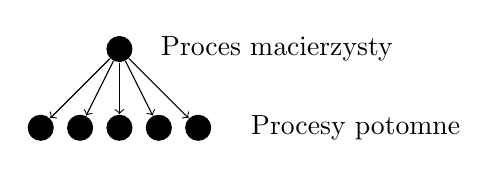
\begin{tikzpicture}
        \node[circle,fill=black] (o)  at ( 0.00, 0.00) {};
        \node[circle,fill=black] (c1) at (-1.00,-1.00) {};
        \node[circle,fill=black] (c2) at (-0.50,-1.00) {};
        \node[circle,fill=black] (c3) at (-0.00,-1.00) {};
        \node[circle,fill=black] (c4) at ( 0.50,-1.00) {};
        \node[circle,fill=black] (c5) at ( 1.00,-1.00) {};
        \node[] at (2.00,0.00) {Proces macierzysty};
        \node[] at (3.00,-1.00) {Procesy potomne};

        \draw[->]  (o) to (c1);
        \draw[->]  (o) to (c2);
        \draw[->]  (o) to (c3);
        \draw[->]  (o) to (c4);
        \draw[->]  (o) to (c5);
      \end{tikzpicture}
      \caption{Hierarchia procesów w~ćwiczeniu 3}
      \label{fig:YT6VA}
    \end{figure}
    %%%%%%%%%%%%%%%%%%%%%%%%%%%%%%%%%%%%%%%%%%%%%%%%%%%%%%%%%%%%%%%%%%%%%

  \item Zadanie jest analogiczne do poprzedniego, z tym, że struktura procesów
    ma wyglądać jak drzewo przedstawione na rysunku \ref{fig:XDQ8Q}.
    %%%%%%%%%%%%%%%%%%%%%%%%%%%%%%%%%%%%%%%%%%%%%%%%%%%%%%%%%%%%%%%%%%%%%
    \begin{figure}[ht]
      \centering
      \begin{tikzpicture}
        \node[circle,fill=black] (c1) at (-1.50, 1.50) {};
        \node[circle,fill=black] (c2) at (-1.00, 1.00) {};
        \node[circle,fill=black] (c3) at (-0.50, 0.50) {};
        \node[circle,fill=black] (c4) at ( 0.00, 0.00) {};

        \node[] at (-1.00, 1.90) {Proces początkowy (,,root'')};
        \node[] at (-0.00,-0.40) {Trzeci potomek};

        \draw[->]  (c1) to (c2);
        \draw[->]  (c2) to (c3);
        \draw[->]  (c3) to (c4);
      \end{tikzpicture}
      \caption{Hierarchia procesów w~ćwiczeniu 4 dla trzech potomków}
      \label{fig:XDQ8Q}
    \end{figure}
    %%%%%%%%%%%%%%%%%%%%%%%%%%%%%%%%%%%%%%%%%%%%%%%%%%%%%%%%%%%%%%%%%%%%%
    Każdy z procesów, oprócz ostatniego tworzy jeden proces potomny.
\end{myenumerate}


\cleardoublepage

%% \label{??:7HOCC}
%% \label{??:3UDS1}
%% \label{??:BYA03}
%% \label{??:LDB7J}
%% \label{??:HXCTX}
%% \label{??:V35FU}
%% \label{??:V285P}
%% \label{??:0DR40}
%% \label{??:TFLMK}
%% \label{??:OD9EZ}
%% \label{??:87ILN}
%% \label{??:HY94T}
%% \label{??:GIWGJ}
%% \label{??:S0ENF}
%% \label{??:5O33M}
%% \label{??:9LCEW}
%% \label{??:FMIVT}
%% \label{??:8O5ZW}
%% \label{??:5GR5X}
%% \label{??:3KG12}
%% \label{??:O26C4}
%% \label{??:QXXWZ}
%% \label{??:FKPAJ}
%% \label{??:IUWYS}
%% \label{??:AKF4R}
%% \label{??:T7RU4}

% vim: set spell spelllang=pl:
